%% Header mit Deklarationen
\documentclass[%
paper=a4,      % alle weiteren Papierformat einstellbar
fontsize=11pt, % Schriftgr��e (12pt, 11pt (Standard))
BCOR1cm,       % Bindekorrektur, bspw. 1 cm
DIV15,         % f�hrt die Satzspiegelberechnung neu aus s. scrguide 2.4
twoside,       % Doppelseiten
headsepline,   %
headings=openright, % Kapitel nur rechts beginnen
%biblography=totoc, % Literaturverzeichnis einf�gen bibtotocnumbered: nummeriert
parskip=half,  % Europ�ischer Satz mit Abstand zwischen Abs�tzen
chapterprefix, % Kapitel anschreiben als Kapitel
headsepline,   % Linie nach Kopfzeile
titlepage,     %
numbers=noenddot,
%draft	       % zeigt �berlange Zeilen an
]{scrreprt}

\usepackage{pdfpages}       % Titelseite hat ein anderes Layout. Sie wird 
                            % separat erzeugt und hier eingef�gt
\usepackage[T1]{fontenc}
\usepackage[utf8,latin1,applemac]{inputenc}  % Zeichencodierung
\usepackage[ngerman, english]{babel} % Worttrennung nach neuer Rechtschreibung
\usepackage{ellipsis}       % Leerraum um Auslassungspunkte
\usepackage{fixltx2e}       % Fehlerkorrektur Zeichens�tze
\usepackage{xspace}         % f�ge evtl. notwendiges Leerzeichen hinzu (\xspace)
\usepackage[]{hyperref}

%\usepackage{mathptmx}           % Times + passende Mathefonts
\usepackage{mathpazo}           % Palatino + passende Mathefonts
\usepackage[scaled=.92]{helvet} % skalierte Helvetica als \sfdefault
\usepackage{courier} 
\usepackage{bm}           % Courier als \ttdefault

\usepackage{graphicx}    % Einbindung von Grafiken
\graphicspath{{bilder/}} % Unterverzeichnis, in dem Grafiken abgelegt werden
\usepackage{listings}    % Listenausgabe externer Dateien

\usepackage{float}      % Paket zum Erweitern der Floatumgebungen
\usepackage[figuresright]{rotating}   % Rotieren von Objekten
%\usepackage{hvfloat}
\usepackage{array}      % Paket zum Erweitern der Tabelleneigenschaften
\usepackage{booktabs}   % Paket f�r sch�nere Tabellen

\usepackage{amsmath}    % erweiterte Mathematik-Umgebungen
\usepackage{amssymb}
\usepackage{cite}

% Einstellungen f�r das Literaturverzeichnis
\usepackage[square,sort,comma,numbers]{natbib}
\setlength{\bibsep}{0.5\baselineskip}
\setlength{\bibhang}{1cm}

% Andere Schriftarten in Koma-Script
\setkomafont{sectioning}{\normalfont\bfseries}
\setkomafont{captionlabel}{\rmfamily\bfseries\small}
\setkomafont{caption}{\mdseries\itshape\small}
\setkomafont{pagehead}{\normalfont\itshape} % Kopfzeilenschrift
\setkomafont{descriptionlabel}{\normalfont\bfseries}

% Kopf und Fu�zeilen
\usepackage[automark]{scrpage2}

% Literaturverzeichnis-Stil
\bibliographystyle{plain}

% weitere Einstellungen
\tolerance=200               % �bervolle Zeile vermeiden
\emergencystretch=3em

\clubpenalty=10000           % 'Schusterjungen' und 'Hurenkinder' vermeiden
\widowpenalty=10000 
\displaywidowpenalty=10000

\parindent 0pt               % Einzug zu Absatzbeginn festlegen

\setcapindent{1em}           % Zeilenumbruch bei Bildbeschreibungen.

\setcounter{secnumdepth}{3}  % Strukturiertiefe bis subsubsection{} m�glich
\setcounter{tocdepth}{3}     % Dargestellte Strukturiertiefe im Inhaltsverzeichnis

% Korrekturversion mit 1.5-fachem Zeilenabstand im Hauptteil:
\newif\ifiscorrect
%\iscorrecttrue   % Korrekturversion
\iscorrectfalse % keine Korrekturversion

%% Eigene Definitionen:

% Einheiten:
\def\ut#1{\ensuremath{\,\mathrm{#1}}}

% Operatoren:
\def\grad{\ensuremath{\mathop{\mathrm{grad}}\nolimits}}
\def\transp#1{\ensuremath{{#1}^\mathsf{T}}}  % transpose
\def\const{\ensuremath{\mathop{\mathrm{const.}}\nolimits}}

% Formelzeichen:
\def\vec#1{\ensuremath{\mathbf{#1}}}
\def\matr#1{\ensuremath{\mathbf{#1}}}

% Hack, um ein zus�tzliches Leerzeichen nach \input zu entfernen:
\def\myinput#1{%
  \endlinechar=-1 % kein Zeilenabschlusszeichen
  \input #1\relax
  \endlinechar `\^^M % Zeilenabschluss = Zeilenvorschub
}

\DeclareOldFontCommand{\bf}{\normalfont\bfseries}{\mathbf}
\begin{document}

% R�mische Nummerierung f�r Sonderseiten, wie Verzeichnisse und Anhang
\selectlanguage{english}
\pagenumbering{Roman}
\pagestyle{plain}

%% Titelblatt

\includepdf[pages=1]{titelseite}
\cleardoublepage

%% Eidesstattliche Erkl�rung
% Die eidesstattliche Erkl�rung mit Unterschrift
\selectlanguage{ngerman}
\chapter*{Erkl"arung der Urheberschaft}

Ich erkl"are hiermit an Eides statt, dass ich die vorliegende Arbeit
ohne Hilfe Dritter und ohne Benutzung anderer als der angegebenen
Hilfsmittel angefertigt habe; die aus fremden Quellen direkt oder
indirekt "ubernommenen Gedanken sind als solche kenntlich gemacht. Die
Arbeit wurde bisher in gleicher oder "ahnlicher Form in keiner anderen
Pr"ufungsbeh"orde vorgelegt und auch noch nicht ver"offentlicht.


\vspace{4cm}

\hspace{2cm} Ort, Datum \hfill Unterschrift \hspace{2cm}

\cleardoublepage

%% Abstract
\begin{abstract}
In recent years, a positive trend of total water storage is detected in many big basins. One of them is Ob river basin in west Siberia, where 27 million people live in 39 cities. In this thesis, measurements from GRACE and GRACE-FO mission are employed and analyzed to determine the total water storage change in this region since 2003. Meanwhile, precipitation and evapotranspiration from global datasets and runoff determined using satellite altimetry will also be taken into discussion to analyze the reasons of the trend. The data from different resources are summarized using Gauss-Markov adjustment. \\\\
It was found that from the launch of GRACE till 2013 the total water storage has slightly decreased, from 2013 to 2015 this catchment has gained water due to increased precipitation and low evapotranspiration. After 2016, total water storage in this area has reduced because the precipitation is lower and the evapotranspiration is stronger.
\end{abstract}
\cleardoublepage

%% Verzeichnisse
% Inhalt Kopf-/Fu�zeile
\pagestyle{scrheadings}
\clearscrheadfoot            % Standardkram wegwerfen
\ohead[\pagemark]{\pagemark} % oben au�en Seitenzahl 
%
% Inhaltsverzeichnis
%
\tableofcontents

%
% Abbildungsverzeichnis
%
\listoffigures

%
% Tabellenverzeichnis
%
\listoftables


% Merke mir die r�mische Seitenzahl in 'roemisch' und setzte Nummeriernung 
% auf arabisch f�r die eigentlichen Kapitel
\cleardoublepage %\newpage
\newcounter{roemisch}
\setcounter{roemisch}{\value{page}}
\pagenumbering{arabic}

\ifiscorrect\linespread{1.5}\selectfont% Zeilenabstand: 1 1/2 (f�r bessere Korrektur)
\else\fi

%% Die einzelnen Kapitel
% Kopfzeile: links Kapitel, rechts Sektion
\clearscrheadfoot            % Standardkram wegwerfen
\ohead[\pagemark]{\pagemark} % oben au�en Seitenzahl 
\ihead{\headmark}            % oben innen automatischer Abschnittsname
%\automark[]{section}
\chapter{Introduction}
\section{Water Cycle}
Water is one of the most necessary resources for human beings. It is the most important ingredient of life; it has a regulating effect on climate and all industries can not function well without it. However, 98 \%
of the water on the earth is in the oceans, 1.6\% is in ice caps, which means only 0.4 \% is the
fresh water on land. So, a very little variability of the hydrology cycle can have big effects on
water resources. \\\\
The hydrology cycle (see figure \ref{fig:hydrologic cycle}) includes 3 major parts: evaporation, precipitation and runoff. The water evaporates from the oceans and the land surface as vapor to become part of the atmosphere along with water from evapotranspiration, which is water transpired from plants and evaporated from the soil and the cooler temperature causes the vapor into clouds. The clouds fall out of the sky as precipitation, which includes rain, snow and ice. Most precipitation falls back into the oceans or onto land. Precipitated water may be intercepted by vegetation, become overland flow over the ground surface, flow through the soil as subsurface flow and discharge into streams as surface runoff. The process can be simplified as:
\begin{equation}
	\frac{dS}{dt} = Pre - ET - R
\end{equation}
where
\begin{table}[htbp]
	\begin{tabular}{ll}
		$Pre$   & Precipitation    \\ 
		$ET$    & Evatranspiration \\ \
		$R$     & Surface Runoff \\ 
		$dS / dt$ & total water storage change \\ 
	\end{tabular}
\end{table}
\begin{figure}[htbp]
	\centering
	
\includegraphics[width=0.7\textwidth]{water-cycle-natural} % Datei in "bilder/" bei LaTeX: eps, bei PDFLaTeX: jpg (o.ä.) 
	\caption{Horologic Cycle} 
	\label{fig:hydrologic cycle}
\end{figure}
\section{Observation from Satellite}
It was extremely difficult to measure the global water storage change consistently. In some way, remote sensing with satellite is the perfect tool for hydrology research, which has the ability to provide the data globally in a long term.\\\\
The GRACE twin satellites, launched 17 March 2002, are making detailed measurements of Earth's gravity field, which are caused by monthly changes in mass. The mass changes can be thought of as concentrated in a very thin layer of water thickness changes near the Earth's surface by moving ocean, atmospheric and land ice masses and by mass exchanges between these Earth system compartments. \\\\
There are 2 satellites with tandem polar orbit. Since the orbit is around the pole and the earth rotates itself, the satellites were able to get the whole view of the earth. Unlike the normal remote sensors, the GRACE satellites measured the gravity field of the earth. When the 2 satellites went over a mass anomaly like a big mountain, the distance of them will be a little bit smaller. By calculating this distance difference with the help of GPS system, the gravity field anomaly of the earth along with the total water storage anomaly are able to be plotted monthly. \\\\
It is shown, that GRACE delivers the highest temporal resolution and is thus able to observe monthly mass variation with a spatial resolution of less than 1000\ut{km}. In (Wahr et al., 1998) it was predicted that GRACE would be able to measure these effects with an accuracy of about 2\ut{mm} of water equivalent heights. Though this accuracy has not yet been achieved because of the errors in spherical harmonic coefficients of short-wavelength, it was shown in many publications that the Stokes coefficients from GRACE indeed contain hydrological signals as the monthly solutions from GRACE showed a good agreement with mass variations from hydrological models.
\begin{figure}[htbp]
	\centering
	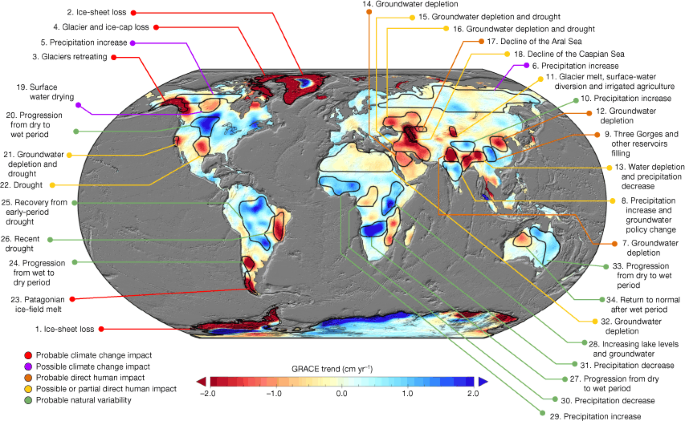
\includegraphics[width=0.6\textwidth]{TWSA} % Datei in "bilder/" bei LaTeX: eps, bei PDFLaTeX: jpg (o.ä.) 
	\caption{Water Storage Change} 
	\label{fig:TWSA}
\end{figure}
\begin{figure}[ht]
	\centering
	
\includegraphics[width=0.6\textwidth]{Obbasin} % Datei in "bilder/" bei LaTeX: eps, bei PDFLaTeX: jpg (o.ä.) 
	\caption{Ob basin} 
	\label{fig:Obbasin}
\end{figure}\\
\section{Motivation}
A time series is a series of data points indexed (or listed or graphed) in time order. Most commonly, a time series is a sequence taken at successive equally spaced points in time. Thus it is a sequence of discrete-time data.  In hydrology, most variables are observed in time series, including Total Water Storage Anomaly(TWSA). In the hydrological cycle, this should reflect seasonal behavior and is in long term relatively stable. However, it was shown that since 2002 the TWSA of many big basins has increased (see figure \ref{fig:TWSA}). One important basin of them is Ob basin in west Siberia (see figure \ref{fig:Obbasin}). How did this trend happen is a very interesting topic. Through the analysis of the trend of the time series, it is possible to further understand the changes that have taken place before and future changes can also be predicted based on the stationary analysis.
\section{Objective}
In this thesis, the beginning point of the changing trend is to be found by analyzing the TWSA time series from GRACE data. In order to find the reason of the change, the precipitation, the evatranspiration along with the runoff in the same period from different data center would also be processed and compared with the TWSA. At the end, how was the changes of the TWSA and the reasons for this change would be discussed. 

\chapter{Study Area}
Ob River (\autoref{fig:Ob Basin}), river of central Russia. One of the greatest rivers of Asia, the Ob flows north and west across western Siberia in a twisting diagonal from its sources in the Altai Mountains to its outlet through the Gulf of Ob into the Kara Sea of the Arctic Ocean. It is a major transportation artery, crossing territory at the heart of Russia that is extraordinarily varied in its physical environment and population. Even allowing for the barrenness of much of the region surrounding the lower course of the river and the ice-clogged waters into which it discharges, the Ob drains a region of great economic potential.\\\\
\begin{figure}[htbp]
	\centering
	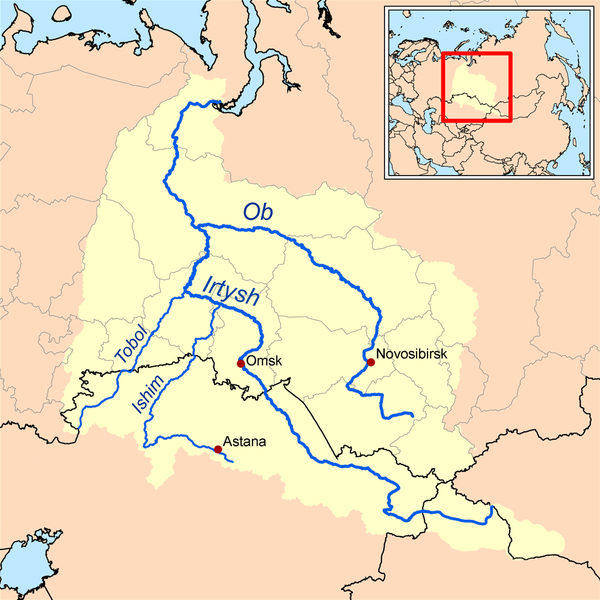
\includegraphics[width=0.7\textwidth]{Obbasin_area} % Datei in "bilder/" bei LaTeX: eps, bei PDFLaTeX: jpg (o.ä.) 
	\caption{River Basins Ob http://www.geologypage.com/2014/03/ob-river.html} 
	\label{fig:Ob Basin}
\end{figure}
\section{Physiography}
The Ob proper is formed by the junction of the Biya and Katun rivers, in the foothills of the Siberian sector of the Altai, from which it has a course of 3 650 km. If, however, the Irtysh River is regarded as part of the main course rather than as the Ob's major tributary, the maximum length, from the source of the Black (Chorny) Irtysh in China's sector of the Altai, is 5 410 km, making the Ob the seventh longest river in the world. The catchment area is approximately 2 975 000 square km. Constituting about half of the drainage basin of the Kara Sea, the Ob's catchment area is the sixth largest in the world. The drainage basin is classified as cropland (36\%), forest (30\%), wetland (11\%), grassland (10\%), shrub (5\%) , developed (5\%) and irrigated cropland (3\%).\cite{revenga1998watersheds}\\\\
The West Siberian Plain covers about 85 percent of the Ob basin.\cite{Obriver} The rest of the basin comprises the terraced plains of Turgay (Kazakhstan) and the small hills of northernmost Kazakhstan in the south and the Kuznetsk Alatau range, the Salair Ridge, the Altai Mountains and their foothills and outliers in the southeast.\\\\
The huge basin of the Ob stretches across a number of natural zones. Semidesert prevails in the far south around Lake Zaysan (recipient of the Black Irtysh and source of the Irtysh proper), bordered on the north by steppe grassland. The central regions of the West Siberian Plain i.e., more than half of the basin-consist of taiga (swampy coniferous forest), with great expanses of marshland. In the north there are vast stretches of tundra (low-lying, cold-tolerant vegetation).
\section{Climate}
\begin{figure}[htbp]
	\centering
	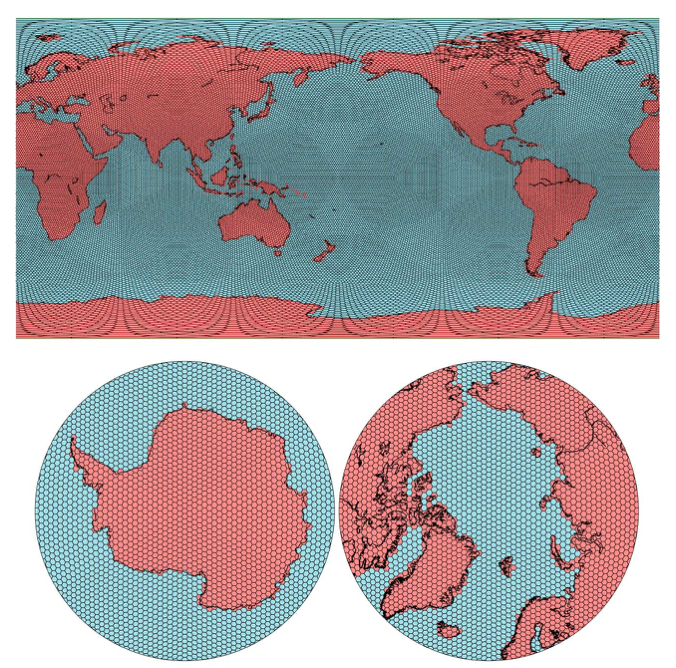
\includegraphics[width=0.5\textwidth]{mascon} % Datei in "bilder/" bei LaTeX: eps, bei PDFLaTeX: jpg (o.ä.) 
	\caption{The distribution of 40,962 geodesic grid tiles over the Earth used as a basis function for estimation of mass
		anomalies from GRACE for CSR mascon solutions. (top) Global view, (bottom left) South Pole view, and (bottom right) North Pole view \cite{save2016high}} 
	\label{fig:mascon}
\end{figure}
The Ob basin has short, warm summers and long, cold winters. Average January temperatures range from  $-28 ^{\circ}$C on the shores of the Kara Sea to $-16 ^{\circ}$C in the upper reaches of the Irtysh. July temperatures for the same locations, respectively, range from 4 $^{\circ}$C to above $20 ^{\circ}$C. The absolute maximum temperature, in the arid south, is $40 ^{\circ}$C,\cite{Obriver} and the minimum, in the Altai Mountains, is $-60 ^{\circ}$. Rainfall, which occurs mainly in the summer, averages less than 400 mm per year in the north, 500 to 600 mm in the taiga zone, and 300 to 400 mm on the steppes. The western slopes of the Altai receive as much as 1 575 mm per year. Snow cover lasts for 240 to 270 days in the north and for 160 to 170 days in the south. It is deepest in the forest zone, where it ranges from 60 to 90 cm, and in the mountains, where it averages 200 cm per year. It is much shallower on the tundra, ranging from 30 to 50 cm, and very thin on the steppe, where 20 to 40 cm fall.\cite{Obriver}\\\\
On the upper Ob the spring floods begin early in April, when the snow on the plains is melting; and they have a second phase, ensuing from the melting of snow on the Altai Mountains. The middle Ob, scarcely affected by the upper Ob's phases, has one continuous spring-summer period of high water, which begins in mid April. For the lower Ob, high water begins in late April or early May. Levels, in fact, begin to rise when the watercourse is still obstructed by ice; and maximum levels, which occur by May on the upper Ob, may not be reached until June, July, or even August on the lower reaches. For the upper Ob, the spring floods end by July, but autumn rains bring high water again in September and October; in the middle and lower Ob, the spring and summer floodwaters gradually recede until freezing sets in. On the lower reaches, flooding may last four months. Flooding of the Ob proper and of the Irtysh obstructs the minor tributaries' drainage.
\section{Hydrology}
The Ob has the third greatest discharge of Siberia's rivers, after the Yenisey and the Lena. On average, it pours some 400 cubic km of water annually into the Arctic Ocean about 12\% of that ocean's total intake from drainage.\\\\
The volume of flow at Salekhard, just above the delta, is about 42 000 cubic metres per second at its maximum and 2 000 cubic metres per second at its minimum, while for Barnaul, on the upper Ob, the corresponding figures are 9 600 and 200 cubic metres per second. The average annual discharge rate at the river's mouth is about 12 700 cubic metres per second. Most of the water comes from the melting of seasonal snow and from rainfall; much less of it comes from groundwater, mountain snow, and glaciers.\cite{Obriver}
\section{Plants and animals}
Pine, cedar, silver fir, aspen, and birch grow on the banks and occasionally constitute isolated forests on the higher ground of the floodplain. Large areas near the river are covered with willow, snowball trees, bird cherry, buckthorn, currant bushes, and wild roses.\\\\
Fur-bearing mammals of the Ob valley include European and Siberian mole, Siberian and American mink, ermine, fox, wolf (in the taiga), elk, white hare, water rat, muskrat, otter, and beaver. Among more than 170 species of birds breeding in the floodplain are grouse, partridge, goose, and duck.
\section{Human use}
Basin total population is about 27 million, with 39 cities having a population of more than 100 000. The Ob's immense hydroelectric potential is estimated at some 250 billion kilowatts. Three main stations have been built: one on the Ob proper, at Novosibirsk, and the other two on the mountainous reaches of the Irtysh, at Bukhtarma and Oeskemen. Both industry and agriculture have been intensively developed in the Ob basin. Cities such as Omsk, Novosibirsk, and Barnaul are major industrial and manufacturing centres. The steppe zone, in the southern Ob basin, is the major producer of spring wheat in Russia. The west Siberian oil and gas fields, located in the taiga and tundra zones of the middle and lower Ob, are the most important in Russia, contributing about two-thirds of the country's crude oil and natural gas output.

\chapter{Data}
\section{GRACE and GRACE-FO}
\subsection{Spherical harmonics}
The variations in the gravity field impacts on both GRACE satellites at different times, such deviations cause a change in the inter-satellite range, which is measured with very high accuracy from the K-band measurement unit. The measured inter-satellite range can be transformed into changes in teh Earth's gravity field, which is described with the Stokes coefficients $\tilde{C}_{lm}$ and $\tilde{S}_{lm}$.\\\\
There is only one Earth gravity field and all centers start off with identical GRACE Level-1 observations, but deriving month-to-month gravity field variations from GRACE observations requires a complex inversion of relative ranging observations between the two formation-flying GRACE spacecraft, in combination with precise orbit determination via GPS and various corrections for spacecraft accelerations not related to gravity changes. Many parameter choices and solution strategies are possible, and have been explored by different data centers. In this thesis the solutions from JPL, CSR, GFZ and ITSG are used, which allows the calculation of gravity filed and equivalent water height anomaly. \autoref{shmethod} shows the method of estimating TWS from GRACE spherical harmonics: 
\begin{equation}
h_{W}(\theta,\lambda;t) = \frac{R \rho_{ave}}{3\rho_{W}} \sum_{l=0}^{\infty} \frac{2l+1}{1+k_{l}} \sum_{m=0}^{l} \tilde{P}_{lm} (\cos \theta) (\Delta \tilde{C} \cos m \lambda + \Delta \tilde{S} \sin m \lambda)
\end{equation}
\subsection{Mass concentration}
Spherical harmonics have been well studied and widely used in satellite geodesy for several decades, based on the computational efficiency of the parameterization, and because the satellite sensitivity is dependent on the spatial wavelength of the mass variations which is implicit in the harmonic basis function. However, unconstrained harmonic solutions from GRACE have typically suffered from poor observability of east-west gradients, resulting in the so-called "stripes" that are conventionally removed via empirical smooting and-or "destriping" algorithms. Although quite effective, especially for larger spatial scales,the destriping also removes some real geophysical signal along with the stripes,and the size shape, and orientation of the signals strongly affect the effectiveness of destriping.\cite{watkins2015improved} \\\\
Thus, to confirm the reliability of spherical harmonic, another common function would be be taken into consideration to estimate mass flux from GRACE, which is called mass concentration(mascon). Each mass tile are defined as a finite truncated spherical harmonic representation up to degree and order 120, which are in turn related to the range-rate observation via their partial derivatives. The size of each tile is aproximately $1^{\circ}$ equatorial longitudinal distance. The mass anomaly for each of the mass tile is estimated using the KBR range-rate observations and the associated spherical harmonic partial derivatives and the singular estimation process is stabilized using Tikhonov regularization solutions with time-variable regularization matrix. \cite{save2016high}. \\\\
This mascon solutions have no stripe errors and capture all the signals ovserved by GRACE within the measurement noise level. The solutions are not tailored for specific applications and are global in nature.\cite{save2016high} 
\begin{figure}[htbp]
	\centering
	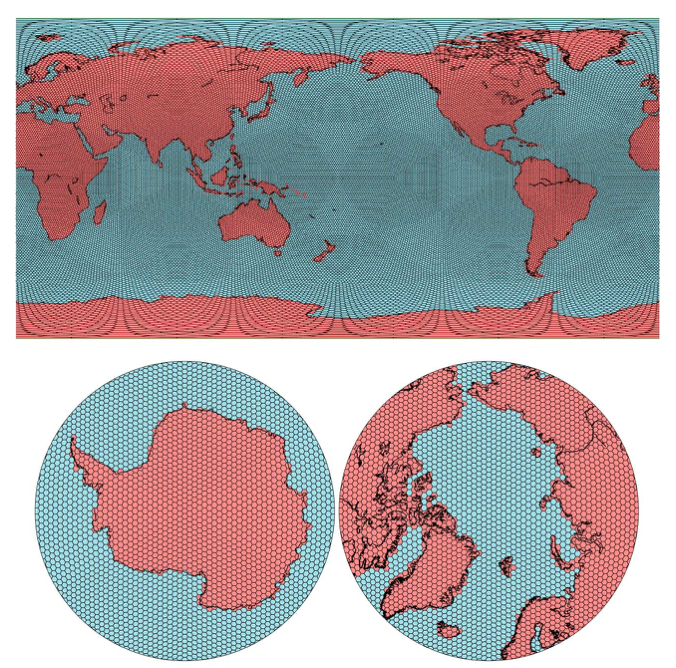
\includegraphics[width=0.5\textwidth]{mascon} % Datei in "bilder/" bei LaTeX: eps, bei PDFLaTeX: jpg (o.ä.) 
	\caption{The distribution of 40,962 geodesic grid tiles over the Earth used as a basis function for estimation of mass
		anomalies from GRACE for CSR mascon solutions. (top) Global view, (bottom left) South Pole view, and (bottom right) North Pole view \cite{save2016high}} 
	\label{fig:mascon}
\end{figure}
In this thesis the mascon solution from CSR are compared with the results from spherical harmonic solutions.
\newpage
\section{Precipitation}
Gauge observations are typically used to measure precipitation directly at the Earth's surface \cite{kidd2001satellite}. Various large-scale climate data sets at different spatiotemporal scales have been developed from station (in situ) observations. These different types of precipitation data product have proved useful across a wide range of fields of research \cite{sun2018review}.
In this thesis the precipitation data from 9 data resources are gathered and processed (\autoref{tab:pre}). The methods dealing with these data sets will be discussed later:
\begin{table}[htbp]\centering 
	\begin{tabular}{|l|l|l|l|l|}
		\hline
		\textbf{Dataset}      & \textbf{Timespan}       & \textbf{Temporal Resolution} & \textbf{Spatial Resolution} & \textbf{Spatial Coverage} \\ \hline
		PREC/L       & 1948 - present & Monthly             & $0.5^{\circ} \times 0.5^{\circ}$          & Global           \\ \hline
		CPC          & 1979 - present & Monthly , Daily    & $0.5^{\circ} \times 0.5^{\circ}$          & Global           \\ \hline
		GPCP         & 1979 - present & Monthly             & $2.5^{\circ} \times 2.5^{\circ}$          & Global           \\ \hline
		CMAP         & 1979 - present & Monthly             & $2.5^{\circ} \times 2.5^{\circ}$          & Global           \\ \hline
		PERSIANN-CDR & 1983 - present & Monthly , Daily    & $0.25^{\circ} \times 0.25^{\circ}$        & $60S^{\circ} - 60N^{\circ}$      \\ \hline
		NCEP1        & 1948 - present & Monthly , Daily    & $2.5^{\circ} \times 2.5^{\circ}$          & Global           \\ \hline
		NCEP2        & 1979 - present & Monthly , Daily    & $1.875^{\circ} \times 1.875^{\circ}$      & Global           \\ \hline
		ERA5         & 1979 - present & Monthly             & $31\ut{km} \times 31\ut{km}$        & Global           \\ \hline
		MERRA-2      & 1980- present  & Monthly , Daily    & $0.5^{\circ} \times 0.625^{\circ}$        & Global           \\ \hline
	\end{tabular}
	\caption{precipitation datasets}
	\label{tab:pre}
\end{table}
\paragraph{Precipitation reconstruction over land (PREC/L)}
PREC/L if provided from National Oceanic and Atmospheric Administration (NOAA).It is derived from gauge observations from over 17 000 stations collected in the Global Historical Climatology Network(GNCN), and the Climate Anomaly Monitoring System(CAMS) datasets. By using OI analysis procedure, the monthly gridded analyses of precipitation over the global land area since 1948 are presented. The mean distribution and annual cycle of precipitation observed in the PREC/L showed good agreement with those in several published gauge-based datasets. \cite{chen2002global}
\paragraph{CPC unified gauge-based analysis of global daily precipitation}
This dataset is provided from Climate Prediction Center(CPC). A gauge-based analysis of daily precipitation has been constructed over the global land areas. Gauge reports from over 30 000 stations are collected from multiple sources including GTS, COOP, and other national and international agencies. Quality control is performed through comparisons with historical records and independent information from measurements at nearby stations, concurrent radar / satellite observations, as well as numerical model forecasts. Quality controlled station reports are then interpolated to create analyzed fields of daily precipitation with consideration of orographic effects \cite{xie2007gauge}. The daily analysis is constructed on a 0.125 degree lat/lon grid over the entire global land areas, and released on a 0.5 degree lat/lon grid over the global domain for a period from 1979 to the present.\cite{xie2010cpc} This dataset has two components: (a) the "retrospective version" which uses 30K stations and spans 1979-2005 and (b) the "real-time version" which uses 17K stations and spans 2006-present.
\paragraph{Global Precipitation Climatology Project (GPCP)}
In this dataset, precipitation data from rain gauge stations, satellites and sounding obsevations have been merged to estimate monthly rainfall on a 2.5 degree global grid since 1979. It provides a consistent analysis of global precipitation from the integration of various satellite data sets of lands and oceans and a gauge analysis over land. 
\paragraph{CPC Merged Analysis of Precipitation (CMAP)}
This data set is also constructed from an analysis of gauge data and satellite-derived precipitation estimates. The overlapping satellite and reanalysis-based estimates are weighted according to their fit with the gauge-based analysis. The quality of this is in general the best in the tropics and weakens towards the polar regions. 
\paragraph{Precipitation Estimation from Remotely Sensed Information using Artificial Neural Networks - Climate Data Record(PERSIANN-CDR)}
This data set provides daily rainfall estimates at a spatial resolution of 0.25 degrees in the latitude band 60S - 60N from 1983 to the near-present. The precipitation estimate is produced using the PERSIANN algorithm on GridSat-B1 infrared satellite data, and the training of the artificial neural network is done using the National Centers for Environmental Prediction (NCEP) stage IV hourly precipitation data. The PERSIANN-CDR is adjusted using the Global Precipitation Climatology Project (GPCP) monthly product.
\paragraph{NCEP/NCAR Reanalysis 1\&2}
The NCEP/NCAR Reanalysis 1 project is using a state-of-the-art analysis/forecast system to perform data assimilation using past data from 1948 to the present. The system has been designed with advanced quality control and monitoring components, and can produce 1 mon of reanalysis per day on a Cray YMP/8 supercomputer. Different types of output archives are being created to satisfy different user needs\cite{kalnay1996ncep}. The NCEP Reanalysis 2 is the improvement of the NECP Reanalysis 1.
\paragraph{ERA5}
ERA5 is produced using 4D-Var data assimilation in CY41R2 of ECMWF's Integrated Forecast System (IFS), with 137 hybrid sigma/pressure (model) levels in the vertical, with the top level at 0.01 hPa. Atmospheric data are available on these levels and they are also interpolated to 37 pressure, 16 potential temperature and 1 potential vorticity level(s). \cite{hersbach2020era5}"Surface or single level" data are also available, containing 2D parameters such as precipitation, 2m temperature, top of atmosphere radiation and vertical integrals over the entire atmosphere. The IFS is coupled to a soil model, the parameters of which are also designated as surface parameters, and an ocean wave model.\\\\
The ERA5 dataset contains one (hourly, 31 km) high resolution realisation (referred to as "reanalysis" or "HRES") and a reduced resolution ten member ensemble (referred to as "ensemble" or "EDA"). Generally, the data are available at a sub-daily and monthly frequency and consist of analyses and short (18 hour) forecasts, initialised twice daily from analyses at 06 and 18 UTC.\cite{hersbach2020era5} Most analysed parameters are also available from the forecasts. There are a number of forecast parameters, e.g. mean rates and accumulations, that are not available from the analyses.
The daily total precipitation can then be calculated from ERA5 data using python with the help of CDS API.
\paragraph{Modern-Era Retrospective analysis for research and Applications, version 2 (MERRA-2)}
This is a global atmospheric reanalysis produced by the NASA Global Modeling and Assimilation Office(GMAO). It spans the satellite observing era from 1980 to the present. The goals of MERRA-2 are to provide a regularly-gridded, homogeneous record of the global atmosphere, and to incorporate additional aspects of the climate system including trace gas constituents (stratospheric ozone), and improved land surface representation, and cryospheric processes.
\section{Evapotranspiration}
Evaporation is the process whereby liquid water is converted to water vapour (vaporization) and removed from the evaporating surface (vapour removal). Water evaporates from a variety of surfaces, such as lakes, rivers, pavements, soils and wet vegetation. 6 datasets are used in this thesis (\autoref{tab:et}). 
\begin{table}[htbp]\centering 
	\begin{tabular}{lllll}
		&                                     &                                          &                                         &                                       \\ \hline
		\multicolumn{1}{|l|}{\textbf{Dataset}}    & \multicolumn{1}{l|}{\textbf{Timespan}}       & \multicolumn{1}{l|}{\textbf{Temporal Resolution}} & \multicolumn{1}{l|}{\textbf{Spatial Resolution}} & \multicolumn{1}{l|}{\textbf{Spatial Coverage}} \\ \hline
		\multicolumn{1}{|l|}{GLDAS NOAH} & \multicolumn{1}{l|}{2000 - present} & \multicolumn{1}{l|}{Monthly}             & \multicolumn{1}{l|}{$0.25^{\circ} \times  0.25^{\circ}$}        & \multicolumn{1}{l|}{$60^{\circ}S - 90^{\circ}N$}      \\ \hline
		\multicolumn{1}{|l|}{GLDAS CLSM} & \multicolumn{1}{l|}{2000 - present} & \multicolumn{1}{l|}{Monthly}             & \multicolumn{1}{l|}{$0.25^{\circ} \times 0.25^{\circ}$}        & \multicolumn{1}{l|}{$60^{\circ}S - 90^{\circ}N$}      \\ \hline
		\multicolumn{1}{|l|}{GLDAS VIC}  & \multicolumn{1}{l|}{2000 - present} & \multicolumn{1}{l|}{Monthly}             & \multicolumn{1}{l|}{$0.25^{\circ} \times 0.25^{\circ}$}        & \multicolumn{1}{l|}{$60^{\circ}S - 90^{\circ}N$}      \\ \hline
		\multicolumn{1}{|l|}{FLDAS}      & \multicolumn{1}{l|}{2002 - present} & \multicolumn{1}{l|}{Monthly}             & \multicolumn{1}{l|}{$0.1^{\circ} \times 0.1^{\circ}$}          & \multicolumn{1}{l|}{$60^{\circ}S - 90^{\circ}N$}      \\ \hline
		\multicolumn{1}{|l|}{SSEBop}     & \multicolumn{1}{l|}{2003- present}  & \multicolumn{1}{l|}{Monthly}             & \multicolumn{1}{l|}{$0.0097^{\circ} \times 0.0097^{\circ}$}    & \multicolumn{1}{l|}{$60^{\circ}S - 60^{\circ}N$}      \\ \hline
		\multicolumn{1}{|l|}{ERA5}       & \multicolumn{1}{l|}{1979 - present} & \multicolumn{1}{l|}{Monthly}             & \multicolumn{1}{l|}{$31\ut{km} \times 31\ut{km}$}            & \multicolumn{1}{l|}{Global}           \\ \hline
	\end{tabular}
	\caption{evapotranspiration datasets}
	\label{tab:et}
\end{table}
\paragraph{The Global Land Data Assimilation System (GLDAS)}
Direct measurements and data acquisition of ET are very difficult and expensive, especially at the global level. Therefore, modeling is one common alternative for estimating ET. GLDAS has been generating quality-controlled, spatially and temporally consistent, terrestrial hydrologic data, including ET and other variants. The goal of GLDAS is to ingest satellite- and ground*based observational data products, using advanced land surface modeling and data assimilation techniques, in order to generate optimal fields of land surface states and fluxes.\\\\
The high-quality, global land surface fields provided by GLDAS support several current and proposed weather and climate prediction, water resources applications, and water cycle investigations. The project has resulted in a massive archive of modeled and observed, global, surface meteorological data, parameter maps, and output which includes 1-degree and 0.25-degree resolution 1948-present simulations of the NOAH, Common Land Model (CLM), Variable Infiltration Capacity Model (VIC), Mosaic, and Catchment Land Surface Models (CLSM). NOAH, CLSM and VIC are used in this thesis. 
\paragraph{Famine Early Warning Systems Network (FEWS NET) Land Data Assimilation System (FLDAS)}
The goal of the FLDAS project is to achieve more effective use of limited available hydroclimatic observations and is designed to be adopted for routine use for FEWS NET decision support. It is a custom instance of the NASA Land Information System (LIS) that has been adapted to work with domains, data streams, and monitoring and forecast requirements associated with food security assessment in data-sparse, developing country settings. Adopting LIS allows FEWS NET to leverage existing land surface models and generate ensembles of soil moisture, ET, and other variables based on multiple meteorological inputs or land surface models.
\paragraph{optiaonal Simplified Surface Energy Balance (SSEBop)}
The SSEBop seTup is based on the Simplified Surface Energy Balance (SSEB) approach with unique parameteriyation for operational application combines ET fractions generated from remotely sensed MODIS thermal imagery, acquired every 8 days, with reference ET using a thermal index approach. The unique feature of the SSEBop parameterization is that it uses pre-defined, seasonally dynamic, boundary conditions that are unique to each pixel for the hot/dry and cold/wet reference points.
\section{Runoff}\label{sec:runoff}
\subsection{Global datasets}
Runoff is quantity of water discharged in surface streams. Runoff includes not only the waters that travel over the land surface and through channels to reach a stream but also interflow, the water that infiltrates the soil surface and travels by means of gravity toward a stream channel (always above the main groundwater level) and eventually empties into the channel. Runoff also includes groundwater that is discharged into a stream; streamflow that is composed entirely of groundwater is termed base flow, or fair-weather runoff, and it occurs where a stream channel intersects the water table.\\\\
The in-situ run off data are from Global Runoff Data Center (GRDC). The GRDC is an international archive of data up to 200 years old, and fosters multinational and global long-term hydrological studies. Originally established three decades ago, the aim of the GRDC is to help earth scientists analyse global climate trends and assess environmental impacts and risks. Operating under the auspices of WMO the database of quality controlled "historical" mean daily and monthly discharge data grows steadily and currently comprises river discharge data of more than 9,900 stations from 159 countries.\\\\
However, the discharge data from GRDC of Ob river are only up to 2010, which doesn't fit the purpose totally. Thus, like precipitation and evapotranspiration, models from different data centers are considered. \autoref{tab:runoff}. But it is shown later, that these datasets are not good enough. 
\begin{table}[htbp]\centering
	\begin{tabular}{llll}
		&                                     &                                          &                                                                                \\ \hline
		\multicolumn{1}{|l|}{\textbf{Dataset}}    & \multicolumn{1}{l|}{\textbf{Timespan}}       & \multicolumn{1}{l|}{\textbf{Temporal Resolution}} & \multicolumn{1}{l|}{\textbf{Spatial Resolution}}  \\ \hline
		\multicolumn{1}{|l|}{GLDAS NOAH} & \multicolumn{1}{l|}{2000 - present} & \multicolumn{1}{l|}{Monthly}             & \multicolumn{1}{l|}{$0.25^{\circ} \times  0.25^{\circ}$}             \\ \hline
		\multicolumn{1}{|l|}{GLDAS CLSM} & \multicolumn{1}{l|}{2000 - present} & \multicolumn{1}{l|}{Monthly}             & \multicolumn{1}{l|}{$0.25^{\circ} \times 0.25^{\circ}$}             \\ \hline
		\multicolumn{1}{|l|}{GLDAS VIC}  & \multicolumn{1}{l|}{2000 - present} & \multicolumn{1}{l|}{Monthly}             & \multicolumn{1}{l|}{$0.25^{\circ} \times 0.25^{\circ}$}              \\   \hline
		\multicolumn{1}{|l|}{ERA5}       & \multicolumn{1}{l|}{1979 - present} & \multicolumn{1}{l|}{Monthly}             & \multicolumn{1}{l|}{$31\ut{km} \times 31\ut{km}$}                      \\ \hline
		\multicolumn{1}{|l|}{HTESSEL}       & \multicolumn{1}{l|}{1979 - 2012} & \multicolumn{1}{l|}{Monthly}             & \multicolumn{1}{l|}{$0.25^{\circ} \times 0.25^{\circ}$}                     \\ \hline
		\multicolumn{1}{|l|}{LISFLOOD}       & \multicolumn{1}{l|}{1980 - 2011} & \multicolumn{1}{l|}{Monthly}             & \multicolumn{1}{l|}{$0.25^{\circ} \times 0.25^{\circ}$}                    \\ \hline
		\multicolumn{1}{|l|}{ORCHIDEE}       & \multicolumn{1}{l|}{1980 - 2014} & \multicolumn{1}{l|}{Monthly}             & \multicolumn{1}{l|}{$0.25^{\circ} \times 0.25^{\circ}$}                      \\ \hline
		\multicolumn{1}{|l|}{PCR-GLOBWB}       & \multicolumn{1}{l|}{1979 - 2012} & \multicolumn{1}{l|}{Monthly}             & \multicolumn{1}{l|}{$0.5^{\circ} \times 0.5^{\circ}$}                      \\ \hline
		\multicolumn{1}{|l|}{SURFEX}       & \multicolumn{1}{l|}{1980 - 2014} & \multicolumn{1}{l|}{Monthly}             & \multicolumn{1}{l|}{$0.25^{\circ} \times 0.25^{\circ}$}                     \\ \hline
		\multicolumn{1}{|l|}{W3RA}       & \multicolumn{1}{l|}{1979 - 2012} & \multicolumn{1}{l|}{Monthly}             & \multicolumn{1}{l|}{$0.5^{\circ} \times 0.5^{\circ}$}                      \\ \hline
		\multicolumn{1}{|l|}{WaterGAP3}       & \multicolumn{1}{l|}{1980 - 2014} & \multicolumn{1}{l|}{Monthly}             & \multicolumn{1}{l|}{$0.25^{\circ} \times 0.25^{\circ}$}                       \\ \hline
	\end{tabular}
	\caption{runoff datasets}
	\label{tab:runoff}
\end{table}
\subsection{Determination from other component}
Runoff can be calculated using terrestrial water balance \autoref{equa:waterbalence} since the other 3 components are obtained. However, this method is proved by \cite{lorenz2014large} not ideal. It combined various datasets and used different metrics to judge the quality of these combinations. It is shown in \autoref{fig:judgerunoff} that even though in some areas like Amazon this method is feasible, for most area, especially for Ob river basin, it is not very ideal. 
\begin{figure}[htbp]\centering
	\begin{minipage}[t]{0.8\textwidth}
		\centering
		\includegraphics[width=1\textwidth]{Ob1} % Datei in "bilder/" bei LaTeX: eps, bei PDFLaTeX: jpg (o.ä.) 
	\end{minipage}
	\begin{minipage}[t]{0.85\textwidth}
		\centering
		\includegraphics[width=1\textwidth]{Ob2} % Datei in "bilder/" bei LaTeX: eps, bei PDFLaTeX: jpg (o.ä.) 
	\end{minipage}
	\begin{minipage}[t]{0.85\textwidth}
		\centering
		\includegraphics[width=1\textwidth]{Ob3} % Datei in "bilder/" bei LaTeX: eps, bei PDFLaTeX: jpg (o.ä.) 
	\end{minipage}
	\caption{various of data combinations are used to estimate the runoff, there are 3 metrics (PBIAS, correlation and NSE wrt. GRDC) to judge the quality of these combinations for Ob basin}
	\label{fig:judgerunoff}
\end{figure}\\\\
In addition, the altimetry measurement using satellite is also taken into consideration since the station for in-situ discharge(Salekhard)(\autoref{fig:Salekhard}) is known. 
\begin{figure}[htbp]
	\centering
	
\includegraphics[width=0.9\textwidth]{salekhard} % Datei in "bilder/" bei LaTeX: eps, bei PDFLaTeX: jpg (o.ä.) 
	\caption{Station Salekhard} 
	\label{fig:Salekhard}
\end{figure}
\subsection{Water level height}
 Among the space-borne sensors, satellite altimetry can provide surface water height successively with repeat periods of 10 and 35 days. Although satellite altimetry was initially designed for oceanography, four decades of altimetry missions have provided an opportunity to study the continental hydrological cycle as well. By using the methods mentioned later, the runoff can be estimated from the satellite water level.\\\\
 Altimetry satellites basically determine the distance from the satellite to a target surface by measuring the satellite-to-surface round-trip time of a radar pulse. However, this is not the only measurement made in the process, and a lot of other information can be extracted from altimetry.\\\\
 The magnitude and shape of the echoes (or waveforms) also contain information about the characteristics of the surface which caused the reflection. The best results are obtained over the ocean, which is spatially homogeneous, and has a surface which conforms with known statistics.
 \paragraph{Envisat}
Envisat (Environmental Satellite) is a large inactive Earth-observing satellite which is still in orbit. Operated by the European Space Agency (ESA), it was the world's largest civilian Earth observation satellite. It was launched on 1 March 2002 aboard an Ariane 5 from the Guyana Space Centre in Kourou, French Guiana, into a Sun synchronous polar orbit at an altitude of $790\pm10$ km. It orbits the Earth in about 101 minutes, with a repeat cycle of 35 days. After losing contact with the satellite on 8 April 2012, ESA formally announced the end of Envisat's mission on 9 May 2012.\\\\
In working towards the global and regional objectives of the mission, numerous scientific disciplines currently use the data acquired from the different sensors on the satellite to study such things as atmospheric chemistry, ozone depletion, biological oceanography, ocean temperature and colour, wind waves, hydrology (humidity, floods), agriculture and arboriculture, natural hazards, digital elevation modelling (using interferometry), monitoring of maritime traffic, atmospheric dispersion modelling (pollution), cartography and study of snow and ice.
\paragraph{SARAL}
SARAL (Satellite with ARgos and ALtiKa) is a cooperative altimetry technology mission of Indian Space Research Organisation (ISRO) and CNES (Space Agency of France). SARAL performs altimetric measurements designed to study ocean circulation and sea surface elevation. The payloads of SARAL are The ISRO built satellite with payloads modules (ALTIKA altimeter), DORIS, Laser Retro-reflector Array (LRA) and ARGOS-3 (Advanced Research and Global Observation Satellite) data collection system provided by CNES was launched by Indian Polar Satellite Launch Vehicle rocket into the Sun-synchronous orbit (SSO). SARAL was successfully launched on 25 February 2013. It will fill the gap between Envisat and the Sentinel 3 mission of the European GMES program.
\paragraph{Sentinel-3}
Sentinel-3 is an Earth observation satellite constellation developed by the European Space Agency as part of the Copernicus Programme. The Sentinel-3 mission's main objective is to measure sea-surface topography, sea- and land-surface temperature and ocean- and land-surface colour with accuracy in support of ocean forecasting systems, and for environmental and climate monitoring. Sentinel-3 builds directly on the heritage pioneered by ERS-2 and Envisat satellites. Near-real time data will be provided for ocean forecasting, sea-ice charting, and maritime safety services on the state of the ocean surface, including surface temperature, marine ecosystems, water quality and pollution monitoring. The satellite orbit provides a 27-day repeat for the topography package, with a 4-day sub-cycle.
\clearpage

\chapter{Method}
\section{Estimating hydrological component from datasets}\label{section:combine}
As mentioned before, the terrestrial water balance can be written as:
\begin{equation}
P - ET - R = \frac{dS}{dt}
\end{equation}
where
\begin{table}[htbp]
	\begin{tabular}{ll}
		$P$   & Precipitation    \\ 
		$ET$    & evapotranspiration \\ \
		$R$     & Surface Runoff \\ 
		$dS / dt$ & total water storage change \\ 
	\end{tabular}
\end{table}\\
For each, time series from different resources are processed using different methods\\\\
 Jet Propulsion Laboratory (JPL), Center for Space Research (CSR), German Research Centre for Geosciences (GFZ) and Institute of Theoretical Geodesy and Satellite Geodesy (ITSG)  post process Level-1 data of GRACE and provide solutions in terms of spherical harmonics. It should be noted that there is a one-year gap between the GRACE and GRACE-FO and several monthly gaps. This one-year gap would be ignored since we are interested in the long term trend and these monthly gaps are dealt using interpolation. For the equivalent water height we use spline interpolation while for uncertainty we use linear interpolation.\\\\
If two known points are given by the coordinates $(x_0,y0)$ and $(x_1,y_1)$, the linear interpolant is the straight line between these points. For a value $x$ in the interval $(x_0,x_1)$, the value $y$ along the straight line is given from the equation of slopes.
\begin{equation}
	y = y_0 + (x-x_0)\frac{y_1-y_0}{x_1-x_0}
\end{equation}
Spline was a term of elastic rulers that were bent to pass through a number of predifined points (knots). The approch to mathematically modelling the shape of such elastic rulers fixed by $n+1$ knots is to interpolate between all the pairs of knots and new point with polynomials. In MatLab, both of these interpolation methods can be finished using function \textit{griddedInterpolant}.\\\\
We have 4 TWSA time series from CSR, GFZ, ITSG and JPL with different uncertainties. To generate one time series of TWSA for further analyse we use Gaus-Markov model.
\subsection{Adjustment using Gauss-Markov model}\label{sec:Gaussmarkov}
Gauss-Markov model is known as the adjustment with observation equations. The model is as follows
\begin{equation}
\bm{y} = \bm{A}\bm{x} + \bm{e}
\end{equation}
where $y$ is a vector of observations, $A$ is the design matrix, $x$ is a vector of unknowns and $e$ is a vector of measurement errors. Define the \textit{Lagrangian} or \textit{cost function};
\begin{equation}
\mathcal{L}_{a}(x) = \frac{1}{2} \bm{e}^T \bm{e}
\end{equation} 
Then, the adjusted observations can be estimated by using least square criterion, the best $x$ can be found with the minimum cost function. The equations can be solved as following:
\begin{align}
&\hat{\bm{x}} = (\bm{A}^T\bm{A})^{-1}\bm{A}^T\bm{y}\\
&\hat{\bm{y}} = \bm{A}\hat{\bm{x}} = \bm{A}(\bm{A}^T\bm{A})^{-1}\bm{A}^T\bm{y}\\
&\hat{\bm{e}} = \bm{y} - \hat{\bm{y}} = [\bm{I} - \bm{A}(\bm{A}^T\bm{A})^{-1}\bm{A}^T]\bm{y}
\end{align}
In many cases, the observations are not equal weighted, which means they have different quality. To solve this problem,  we use a matrix $\bm{P}$ to describe the weight. The cost function is formed as:
\begin{equation}
\mathcal{L}_{a}(x) = \frac{1}{2} \bm{e}^T \bm{P}\bm{e}
\end{equation}
the weighted least squares estimations are:
\begin{align}
\label{equa:guass0}
&\hat{\bm{x}} = (\bm{A}^T \bm{P}\bm{A})^{-1}\bm{A}^T\bm{P}\bm{y}\\ 
&\hat{\bm{y}} = \bm{A}\hat{\bm{x}} = \bm{A}(\bm{A}^T\bm{P}\bm{A})^{-1}\bm{A}^T\bm{P}\bm{y}\\
&\hat{\bm{e}} = \bm{y} - \hat{\bm{y}} = [\bm{I} - \bm{A}(\bm{A}^T\bm{P}\bm{A})^{-1}\bm{A}^T\bm{P}]\bm{y}
\end{align}\\
For each month, their are 4 EWH values $S_{CSR}(t)$, $S_{GFZ}(t)$, $S_{ITSG}(t)$, $S_{JPL}(t)$ along with their uncertainty $\sigma_{CSR}(t)$, $\sigma_{GFZ}(t)$, $\sigma_{ITSG}(t)$, $\sigma_{JPL}(t)$. We use the uncertainty to build the weight matrix $\bm{P}$, then we have:
\begin{align}
\bm{y} &= \begin{pmatrix} \label{equa:guass1}
S_{CSR}(t)\\
S_{GFZ}(t)\\
S_{ITSG}(t)\\
S_{JPL}(t)
\end{pmatrix} \\
\bm{P} &= \begin{pmatrix} \label{equa:guass2}
\frac{1}{\sigma^2_{CSR}(t)} & 0 & 0 & 0 \\
0 & \frac{1}{\sigma^2_{GFZ}(t)} & 0 & 0 \\
0 & 0 & \frac{1}{\sigma^2_{ITSG}(t)} & 0 \\
0 & 0 & 0 & \frac{1}{\sigma^2_{JPL}(t)}
\end{pmatrix}\\
\bm{A} &= \begin{pmatrix} \label{equa:guass3}
1\\
1\\
1\\
1
\end{pmatrix}
\end{align}
By inserting \autoref{equa:guass1}, \autoref{equa:guass2} and \autoref{equa:guass3} into \autoref{equa:guass0} we are able to get one TWSA for one month
\begin{equation} \label{equa:finalgauss}
\underset{1 \times 1}{\hat{\bm{x}}} = (\underset{1 \times 4}{\bm{A}}^T \underset{4 \times 4}{\bm{P}} \  \underset{4 \times 1}{\bm{A}})^{-1} \underset{1 \times 4}{\bm{A}}^T \underset{4 \times 4}{\bm{P}} \  \underset{4 \times 1}{\bm{y}}
\end{equation}
where $\hat{\bm{x}}$ is the EWH for one month. By repeating \autoref{equa:finalgauss}, we are able to get one whole time series for equivalent water height. The uncertainty for this new time series would be calculated using least squares error:
\begin{equation}
	\sigma(t) = \frac{1}{4}\sqrt{\sigma^2_{CSR}(t)+\sigma^2_{GFZ}(t)+\sigma^2_{ITSG}(t)+\sigma^2_{JPL}(t)}
\end{equation}
The derivation of the TWSA would be calculated using central difference:
\begin{align}\label{eq:dsdt}
\frac{dS(t)}{dt} = &\frac{(dS(t+\Delta t) - dS(t)) + (dS(t) - dS(t-\Delta t))}{2 \Delta t}\\
= & \frac{dS(t+\Delta t) - dS(t-\Delta t)}{2 \Delta t}
\end{align}
where $\Delta t$ is one month. 
The method used in \autoref{sec:Gaussmarkov} also works for precipitation, evapotranspiration and runoff. However, the uncertainties of these time series were unknown. Therefor, it's necessary to get the uncertainty before the adjustment. \\\\
We assume that the precipitation and evapotranspiration are normal distributed during 2002 to 2020 (though it is not the case). Under this assumption, the precipitation and evapotranspiration in the same month every year can be regarded as a constant with random errors. We then can use the standard deviation as the uncertainty.
\begin{gather}
\sigma_{Pre_{Jan}} = \sqrt{\frac{\sum_{i=1}^{n} (Pre(i)_{Jan} - \bar{Pre}_{Jan})}{n-1}}
\end{gather}
where $\sigma_{Pre_{Jan}}$ is the standard deviation of the Precipitation in January, $Pre(i)_{Jan}$ is the precipitation in January in different years and $\bar{Pre}_{Jan}$ is the mean of all the precipitation in January. With the same method we are able to obtain the uncertai nty for precipitation and evapotranspiration in other eleven months. \\\\
The changing points can be found using moving average (MA). In statistics, a moving average is a calculation used to analyze data points by creating a series of averages of different subsets of the full data set. The reason for calculating the moving average is to help smooth out the data by creating a constantly updated average data. In MatLab, this could be down with \textit{movmean} function. The size of subsets is 12 in this thesis because of the number of months in one year.\\\\
After moving average time series the abrupt changes in the mean of the this new series, the sudden change of the time series can be found. This can be achieved using MatLab function \textit{ischange}, which enables user to find the abrupt changes of the a vector in mean value, variance or sloe and intercept. 
\section{Estimating the quality of runoff datasets}\label{sec:runoffdata}
It was mentioned in \autoref{sec:runoff} that the in-situ runoff data existed til 2010, which allows us to estimate the quality of the data models. First, we calculate the diFference between the model and the in-situ data.
\begin{equation}
	d(t) = R(t)_{insitu} - R(t)_{model}
\end{equation}
By plotting the cumulative distribution function (CDF) of $d$, the quality of the model can be estimated. By setting the appropriate quantile we are able to decide if a data model is good enough for further analyze. In this work 10\% of the mean in-situ data are set.  
\section{Estimating the runoff using quantile function and water level}\label{sec:waterlevel}
The river discharge at the selected gauges is typically determined from an empirical functional relation between water level estimated by satellite altimetry and measured discharges. This relation, referred to as a rating curve, is specific to each gauging station and location of altimetry. However, this technique has many limitations. First, first, this technique is limited by the availability of in situ discharge measurements simultaneous with altimetry data. Second, the location of the altimetry foot- print can also limit the usage of the technique.\\\\
Fortunately, \cite{tourian2013quantile} provides a methods, which can represent a direct connection between the quantile functions at the corresponding probability and the relationship between runoff and water level. \\\\
first, we get the quantile functions for altimetric water level,$Q_R(p)$ and discharge from in situ measurement, $Q_W(p)$:
\begin{gather*}
	Q_R(p) = \inf(X_R \in R: p\leq F(X_R)) \\
	Q_W(p) = \inf(X_W \in R: p\leq F(X_W)) 
\end{gather*}
where $X_R$ and $X_W$ refer to the runoff and water level values and $F$ represents the CDF. The quantile function specifies, for a given probability $0 < p < 1$, the maximum value that $X_R$ or $X_W$ can attain with that probability.\\\\
By achieving the function $T$ between the quantile functions, we can get the function between the runoff and water level since $T$ is a non decreasing function. 
\begin{equation}
	Q_R = T(Q_W) \Longrightarrow X_R = T(X_W)
\end{equation}
In principle, the obtained relationship can be used as look-up table implying the desired rating curve. However, as this study aims to compare the statistical and empirical rating curves, a similar way of approximation for both is needed. In this thesis, the simple quadratic estimation is used for modeling the rating curve. Thus, the statistical rating curve is achieved by fitting a quadratic curve over the obtained statistical relationship. \autoref{fig:wltodischarge} showed an example of achieving the runoff using water level data from Envisat. 
\begin{figure}[htbp]
	\centering
	\begin{minipage}[t]{0.45\textwidth}
		\centering
		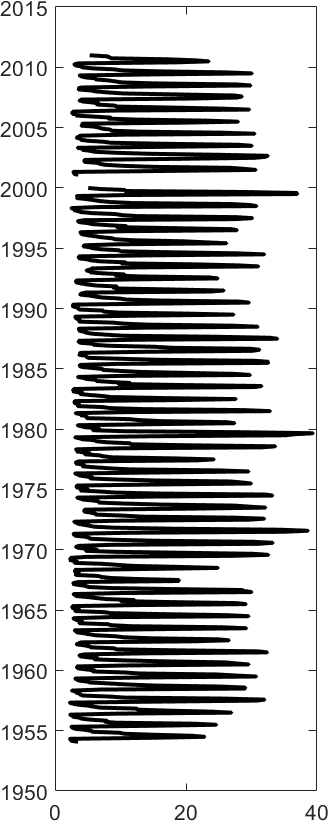
\includegraphics[width=0.4\textwidth]{leftinsitu} % Datei in "bilder/" bei LaTeX: eps, bei PDFLaTeX: jpg (o.ä.) 
	\end{minipage}
	\begin{minipage}[t]{0.45\textwidth}
		\centering
		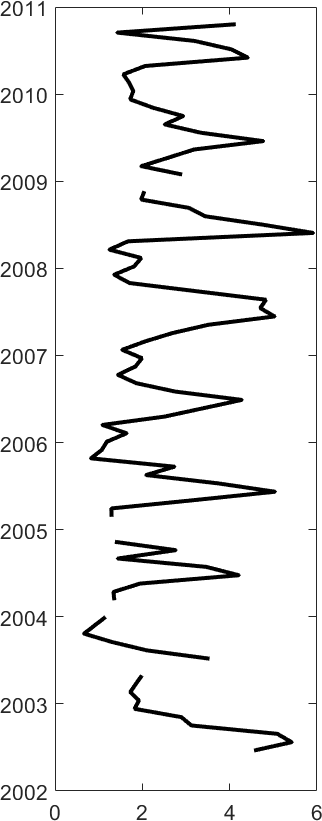
\includegraphics[width=0.4\textwidth]{rightwl} % Datei in "bilder/" bei LaTeX: eps, bei PDFLaTeX: jpg (o.ä.) 
	\end{minipage}
	\begin{minipage}[t]{0.45\textwidth}
		\centering
		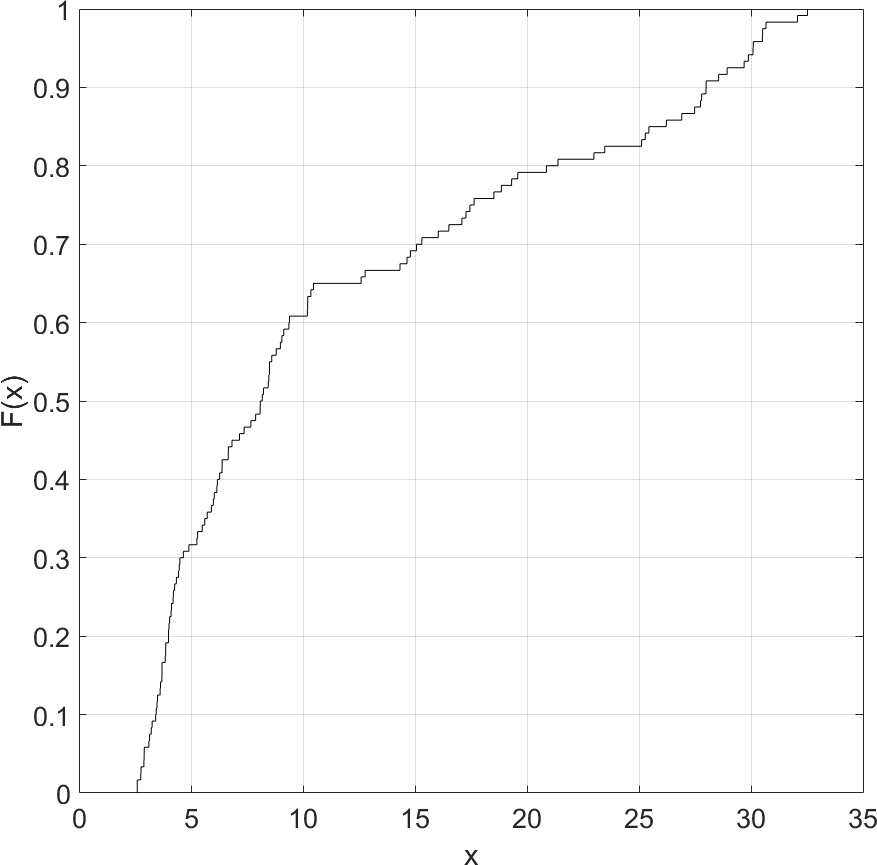
\includegraphics[width=0.7\textwidth]{cdfleft} % Datei in "bilder/" bei LaTeX: eps, bei PDFLaTeX: jpg (o.ä.) 
	\end{minipage}
	\begin{minipage}[t]{0.45\textwidth}
		\centering
		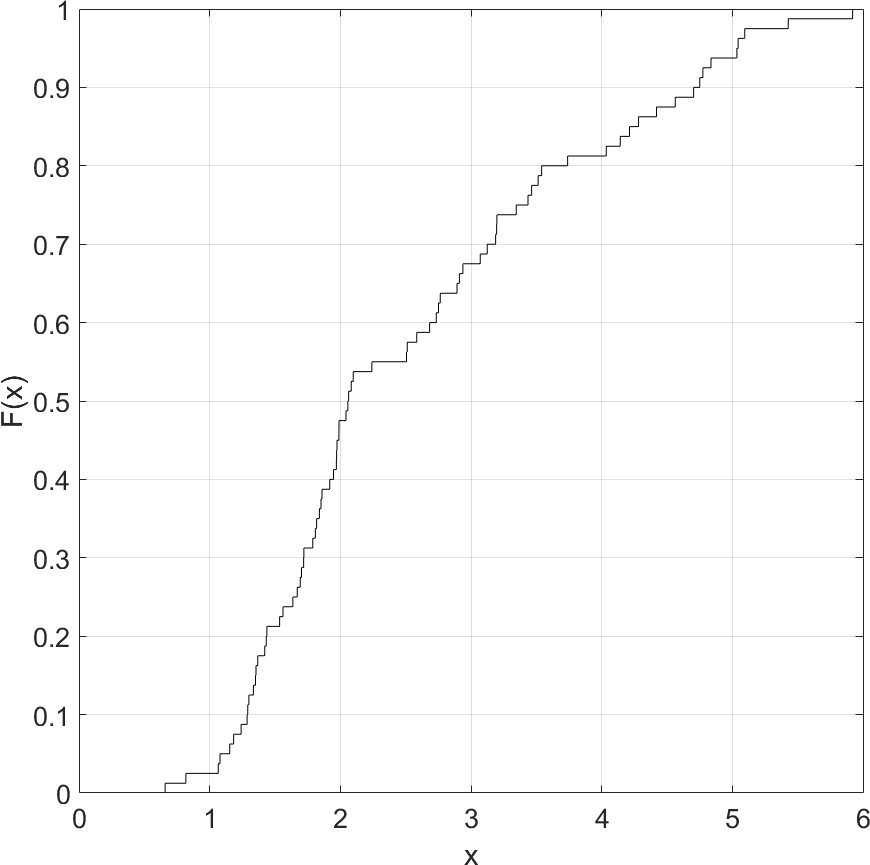
\includegraphics[width=0.7\textwidth]{cdfright} % Datei in "bilder/" bei LaTeX: eps, bei PDFLaTeX: jpg (o.ä.) 
	\end{minipage}
	\begin{minipage}[t]{0.45\textwidth}
		\centering
		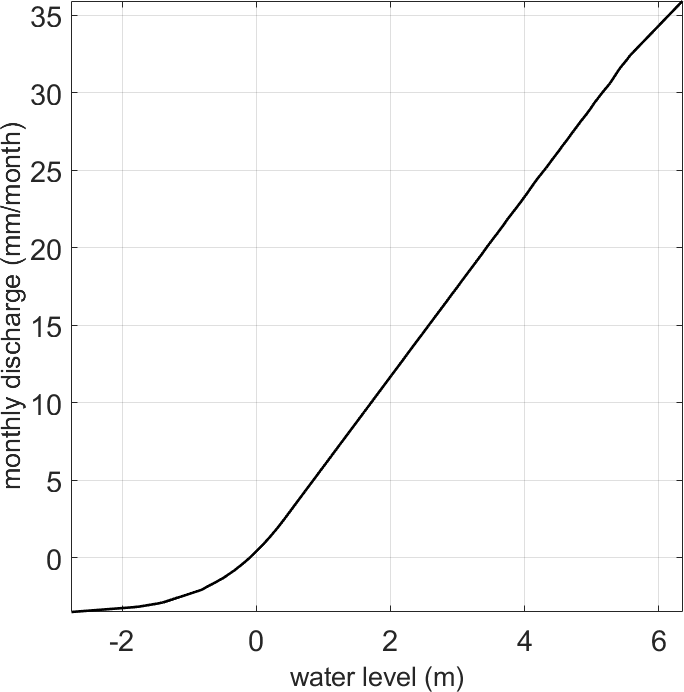
\includegraphics[width=0.7\textwidth]{cdfcombine} % Datei in "bilder/" bei LaTeX: eps, bei PDFLaTeX: jpg (o.ä.) 
	\end{minipage}
	\caption{Available in-situ runoff for Ob river (top left), stimatEd water level from Envisat (top right), and quantile function of water level and runoff (middle). A smoothened rating curve is obtained from the corresponding probabilities (bottom)}
	\label{fig:wltodischarge}
\end{figure}\\\\
By repeating this process to SARAL and Sentinel missions we can generate an whole runoff time series from 2002 to 2020. (note there is a 32 months gap between Envisat and SARAL from November of 2010 to July of 2013) 
\ifiscorrect\linespread{1.0}\selectfont% Zeilenabstand wieder auf 1 zur�ck
\else\fi

% Setze Numerierung wieder auf r�misch zur�ck und setzte von oben fort
% Wert ist demnach der von 'roemisch'
\newpage
\pagenumbering{Roman}
\setcounter{page}{\value{roemisch}}

%% Literaturverzeichnis
\bibliography{literatur/bib}


%% Appendix, falls vorhanden
\appendix
\chapter{Estimating TWS from GRACE SH}\label{shmethod}
The shape of the geoid, i.e. the distance between the reference ellipsoid and the geoid surface $N$, can be expanded in a sum of spherical harmonics.
\begin{equation}
N(\theta, \lambda) = R \sum_{l=0}^{\infty} \sum_{m=0}^{l} \tilde{P}_{lm}(\cos \theta)(\tilde{C}_{lm} \cos m\lambda + \tilde{S}_{lm}\sin m\lambda)
\end{equation}
where
\begin{table}[htbp]
	\begin{tabular}{ll}	
		$N(\theta, \lambda)$	&  geoid height at a point with the spherical coordinates $\theta$,$\lambda$\\ 
		$R$	&  radius of the Earth\\ 
		$\tilde{P}_{lm}$	&  normalized associated Legendre functions of degree $l$ and order $m$\\ 
		$\tilde{C}_{lm}$,$\tilde{S}_{lm}$	&  normalized Stokes coefficients\\ 
	\end{tabular}
\end{table}
The time-dependent change in the geoid heights $\Delta N$ is reflected by the difference between the spherical harmonic coefficients $\tilde{C}_{lm}$,$\tilde{S}_{lm}$. In this case, the equation can be written as:
\begin{equation}
\Delta N(\theta, \lambda) = R \sum_{l=0}^{\infty} \sum_{m=0}^{l} \tilde{P}_{lm}(\cos \theta)(\Delta \tilde{C}_{lm} \cos m\lambda + \Delta \tilde{S}_{lm}\sin m\lambda)
\end{equation}
By assuming that $\Delta N(\theta, \lambda;t) \neq 0$, it is clear that there had to be a change in the Earth's gravity field caused by mass fluctuations in, on and above the Earth's surface. This change is denoted as a change in the Earth's density distribution. In\cite{wahr1998time}, it was found that there is a connection between this quantity and its representation in spherical harmonic coefficients.
\begin{equation}
\begin{Bmatrix}
\Delta \tilde{C}_{lm}(t)\\
\Delta \tilde{S}_{lm}(t)
\end{Bmatrix} = \frac{3}{4\pi R \rho_{ave}(2l+1)} \int \int \Delta \rho(r,\theta,\lambda;t) \tilde{P}_{lm}(\cos \theta) \times (\frac{r}{R})^{l+2} \begin{Bmatrix}
\cos m\lambda \\
\sin m\lambda
\end{Bmatrix} \sin\theta d\theta d\lambda
\end{equation}
where $r$ is the distance of the computation point from the center of the Earth and $\rho_{ave}$ is the average density of the Earth. However, an accurate determination of $\Delta \rho(r,\theta,\lambda;t)$ is nearly impossible, because it requires prior knowledge about the inner density distribution of the Earth. But all short periodic mass variations can be assumed to happen only in a thin layer on the Earth's surface, which can be detected by GRACE satellites. The thickness is mostly determined by the thickness of the atmosphere and is of the order of 10 to 15 \ut{km} \cite{wahr1998time}. \\\\
The change in this thick layer is called surface density $\Delta \rho_{S}$, which can be defined as the radial integral of $\Delta \rho$ through this layer and since the layer is thick enough, it can be assumed that $r \approx R$, so the equation can be simplified as
\begin{equation}
\begin{Bmatrix}
\Delta \tilde{C}_{lm}(t)\\
\Delta \tilde{S}_{lm}(t)
\end{Bmatrix}_{\text{surf mass}} = \frac{3}{4\pi R \rho_{ave}(2l+1)} \int \int \Delta \rho(\theta,\lambda;t) \tilde{P}_{lm}(\cos \theta)  
\begin{Bmatrix}
\cos m\lambda \\
\sin m\lambda
\end{Bmatrix} \sin\theta d\theta d\lambda
\end{equation}
This equation now connects the density redistribution in this thin layer with the spherical harmonic coefficients. Thus, it describes the contribution to the geoid from the direct gravitational attraction of the surface mass \cite{wahr1998time}. The mass fluctuations on the surface also deform the underlying Earth, which implicates a change in the gravitational potential, and thus a change in the geoid shape, as well. This effect is considered by the so called $Love\ number\ k_{l}$, which were derived from\cite{han1995viscoelastic}. The contribution from the deformed solid earth may then be written as
\begin{equation}
\begin{Bmatrix}
\Delta \tilde{C}_{lm}(t)\\
\Delta \tilde{S}_{lm}(t)
\end{Bmatrix}_{\text{solid Earth}} = \frac{3k_{l}}{4\pi R \rho_{ave}(2l+1)} \int \int \Delta \rho(\theta,\lambda;t) \tilde{P}_{lm}(\cos \theta) 
\begin{Bmatrix}
\cos m\lambda \\
\sin m\lambda
\end{Bmatrix} \sin\theta d\theta d\lambda
\end{equation}
The total geoid change is obtained by adding (3.4) and (3.5)
\begin{equation}
\begin{Bmatrix}
\Delta \tilde{C}_{lm}(t)\\
\Delta \tilde{S}_{lm}(t)
\end{Bmatrix} = \begin{Bmatrix}
\Delta \tilde{C}_{lm}(t)\\
\Delta \tilde{S}_{lm}(t)
\end{Bmatrix}_{\text{surf Earth}} + \begin{Bmatrix}
\Delta \tilde{C}_{lm}(t)\\
\Delta \tilde{S}_{lm}(t)
\end{Bmatrix}_{\text{solid Earth}}
\end{equation}
Inserting (3.6) into (3.2) leads to the so called \textit{isotropic transfer coefficients}, which define the quantity of a spherical harmonic series expansion. In the case of a surface mass density, they are defined as 
\begin{equation}
\Lambda_{l} = \frac{R\rho_{ave}}{3} \frac{2l+1}{1+k_{l}}
\end{equation} 
Then an expression for the surface mass density in terms of the spherical harmonic coefficients can be written as
\begin{equation}
\Delta \rho_{S}(\theta,\lambda) = \frac{R \rho_{ave}}{3} \sum_{l=0}^{\infty} \frac{2l+1}{1+k_{l}} \sum_{m=0}^{l} \tilde{P}_{lm} (\cos \theta) (\Delta \tilde{C} \cos m \lambda + \Delta \tilde{S} \sin m \lambda)
\end{equation}
The gravity field change can be assumed as the change of the thin layer of water on the Earth's surface. The relation between the water equivalent heights and the surface mass density is
\begin{equation}
h_{W}(\theta,\lambda) = \frac{\Delta \rho_{S}(\theta,\lambda)}{\rho_{W}}
\end{equation}
where $\rho_{W}$ is the average density of water and thus
\begin{equation}
h_{W}(\theta,\lambda;t) = \frac{R \rho_{ave}}{3\rho_{W}} \sum_{l=0}^{\infty} \frac{2l+1}{1+k_{l}} \sum_{m=0}^{l} \tilde{P}_{lm} (\cos \theta) (\Delta \tilde{C} \cos m \lambda + \Delta \tilde{S} \sin m \lambda)
\end{equation}
For simplicity, this formula can be written as 
\begin{equation}
h_{W}(\theta,\lambda;t) = \sum_{l=0}^{\infty} \Lambda_{l} \sum_{m=0}^{l} \tilde{Y}_{lm}(\theta,\lambda) \Delta \tilde{K}_{lm}(t)
\end{equation}
where 
\begin{itemize}
	\item $\Lambda_{l} = \frac{R \rho_{ave}}{3 \rho w} \frac{2l+1}{1+k_{l}}$: isotropic spectral transfer coefficients
	\item $\tilde{Y}_{lm}(\theta,\lambda) = \tilde{P}_{lm}(\cos \theta)(\cos m\lambda \quad \sin m \lambda)^{T}$: normalized surface spherical harmonics
	\item $ \Delta \tilde{K}_{lm}(t) = (\Delta \tilde{C}_{lm} \quad \Delta \tilde{S}_{lm})^{T}$: normalized Stokes coefficients
\end{itemize}
The associated Legendre functions are given by
\begin{equation}
\tilde{P}_{n,m}(t) = \sqrt{(2-\delta_{m0})(2n+1)\frac{(n-m)!}{(n+m)!}}\sqrt{1-t^2}^{m}\frac{d^{n+m}}{dt^{n+m}}\frac{1}{2^n n!}(t^2 - 1)^n
\end{equation}
where $n$ is degree, $m$ is order and $t= \cos \theta$ is a substitution. The Legendre functions can be calculated by the recursion.
\begin{gather}
\tilde{P}_{0,0}(t) = 1 \\
\tilde{P}_{m,m}(t) = W_{m,m}\sin \theta \tilde{P}_{m-1,n-1}(t-1) \quad  \text{for $m > 0$ and $m =n$} \\
\tilde{P}_{n,m} = W_{n,m}[\cos \theta \tilde{P}_{n-1,m}(t) - \frac{1}{W_{n-1,m}} \tilde{P}_{n-2,m}(t)] \quad \text{for $m \neq n$}
\end{gather}       
with the factors
\begin{equation}
W_{n,m} = \begin{cases}
\sqrt{3} & \text{for $n = 1$ and $m = {0,1}$}\\
\sqrt{\frac{2n+1}{2n}} & \text{if $n=m$ and $n>1$} \\
\sqrt{\frac{(2n+1)(2n-1)}{(n+m)(n-m)}} & \text{$n>1$ and $m \neq n$}
\end{cases}
\end{equation}                   
and the convention $\tilde{P}_{n,m}(t) = 0$ for  $m>n$. This algorithm is shown to be stable until degree $n \approx 1800$. In this thesis they are up to 96. \\\\
It is obvious that only $\Delta \tilde{K}_{lm}$ is time dependent while $\Lambda_{l}$ and $\tilde{Y}_{lm}(\theta,\lambda)$ are constant in time, by using the methods of forwards and backward-differences a rate of mass variations in terms of water equivalent heights can be obtained.
\begin{equation}
\dot{h}_{W}(\theta,\lambda;t) = \sum_{l=0}^{\infty} \Lambda_{l} \sum_{m=0}^{l} \tilde{Y}_{lm}(\theta,\lambda) \Delta \dot{\tilde{K}}_{lm}(t)
\end{equation}
This computation of the area weighted rate of change of water equivalent heights ofr one particular region $\chi$, defined by a set of $k$ grid cell centers $(\theta_{i}, \lambda_{i}),j=1,2,3\cdots,k$, can be done according to
\begin{equation}
\dot{h}_{W}(\chi;t) = \sum_{j=1}^{k}\ \frac{a(\theta_{i},\lambda_{i})}{a(\chi)} sum_{l=0}^{\infty} \Lambda_{l} \sum_{m=0}^{l} \tilde{Y}_{lm}(\theta_{i},\lambda_{i}) \Delta \dot{\tilde{K}}_{lm}(t)
\end{equation}
\begin{table}[htbp]
	\begin{tabular}{ll}
		$\dot{h}_{W}(\chi;t)$	&  rate of mass change in catchment $\chi$\\ 
		$k$	&  number of date points in the catchment\\ 
		$a(\theta_{i},\lambda_{i})$	&  area of the grid cell $j$\\ 
		$a(\chi)$	&  total area of the catchment $\chi$\\ 
	\end{tabular}
\end{table}
In this thesis, the size of the cell is $0.5^{\circ} \times 0.5^{\circ}$, which means there are $360 \times 720$ cells.
With the help of the \textit{shbundle}, \textit{EWHbundle} and the basin mask from the Institute of Geodesy (GIS), University of Stuttgart, this process can easily be done and the equivalent water heights of Ob area between 2002 and 2020 are acquirable. 

\end{document}
